\begin{lemma}
    [Жордана]
    Пусть $f$ непрерывна в $|z| > R_0, \Im z > 0 \}$.
    $M(R) = \sup\left\{ |f(z) ~:~ z : |z| = R, \Im z \geqslant \right\}|$, $\Gamma _R = \{ |z | = R, \Im z \geqslant 0\}$

    Если $M(R) \to 0$, то $\forall m > 0 ~~~\int_{\Gamma_R} f(z) e ^{\Im z dz} \underset{R \to +\infty}{\to} 0 $.

\end{lemma}
% какое-то доказательство

\begin{lemma}
    [О полувычите]

   Пусть $\Gamma = \{ a + r  e ^{i\phi } _{\phi \in [\phi_0, \phi_0 + \pi]}$.
   $a \in \C$~--- простой полюс $f(x)$.

   Тогда $\int_{\Gamma(r)} f (z) dz \underset{r \to 0_+}{\to} \pi i res_a f $.
\end{lemma}

\begin{proof}

    При достаточно малых $r$, т.к. $a$ -- простой множитель
    \begin{align*}
        \int_{\Gamma(r)} f(z)dz &= \int_{\Gamma(r)} \frac{C_{-1}}{z-a} + \overbrace{\sum_{k=0}^{\infty } C_k (z-a)^k}^{\varphi(z)} dz\\
        &= \overbrace{C_{-1}}^{\res_a f} \underbrace{\int_{\Gamma(r)}}_{I_1} \frac{dz}{z-a}  + \overbrace{\int_{\Gamma(r)}\varphi(z) dz}^{J}\\
        I_1 &= \int_{\varphi_0}^{\varphi_0 + \pi} \frac{ire^{i\varphi}d\varphi}{re^{i\varphi}} = \pi i \\
        |J| \leqslant C\cdot \pi r \to 0\quad r\to 0
    .\end{align*}
\end{proof}


\section{Интегралы в смысле главного значния}
Пусть $f \in C\left([a, b] \setminus c) \right)$, $c \in (a, b)$.

\[
v.p. \int_a^b f(x) dx  = \lim_{\varepsilon \to 0^+ } \left(
    \int_a^{c - \varepsilon} f(x) dx + \int_{c + \varepsilon}^b f(x)dx \right).
\]

Особенных точек может быть много, поэтому там может возникнуть нескольк таких пределов.

\begin{example}
    $\int_0^{+\infty} \dfrac{\sin x}{x} dx = I$.

    \begin{align*}
        I &= \dfrac{1}{2} \int_{-\infty}^{infty} \frac{\sin x}{x} \\
        &= \frac{1}{2} v.p. \int _{-\infty }^{\infty } \frac{\overbrace{\sin x}^{\Im e^{ix}}}{x}dx\\
        &= \frac{1}{2} v.p. \frac{1}{i} \int_{-\infty }^{\infty } \frac{\cos x + i\sin x}{x}dx\\
        &= \frac{1}{2i} \pi i = \frac{\pi}{2}\\
    .\end{align*}


    $\frac{\cos x}{x}$ -- нечётная функция, значит интеграл в смысле главного значения по области без особых точек сходится и равен 0.
\end{example}


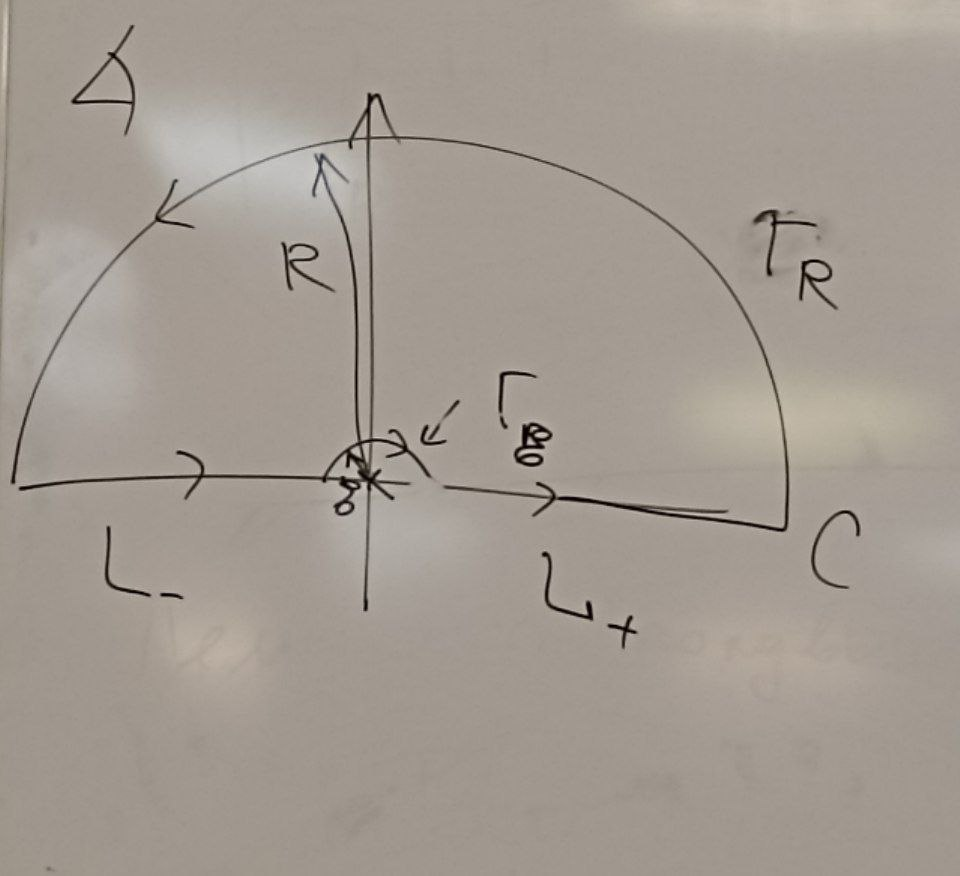
\includegraphics[scale=0.17]{img/obgod_vp.jpg}

$\sphericalangle $ контур из двух верхних полуокружностей с радиусами $R,\varepsilon$ и прямыми вдоль оси $Ox$, соединяющими их, обходимый против часовой стрелки.

\begin{align*}
    0 = \int _C \frac{e^{iz}}{z}dz = \underbrace{\int_{\Gamma_R}fdz}_{\to 0 \text{;Жордан}} + \overbrace{\int_{\Gamma_{\varepsilon}}fdz}^{-\pi i \res_0 f} + \int _{L_+}fdz + \int_{L_-}fdz\\
    v.p. \int_{-\infty }^{\infty }f(x)dx = \pi i \res_0f = \pi i
.\end{align*}


\section{Возвращение к дифферецниальным формам}

\begin{definition}
    $\omega$ -- замкнутая формула если $d\omega = 0$
\end{definition}

\begin{definition}
    $\omega$ -- точная в области $O$, если существует форма $\Omega$ -- дифферецниальная форма в области $O$, т.ч. $d\Omega = \omega$
\end{definition}

\begin{lemma}
    Точноасть влечёт засмкнутость. Потому что $d(d(\Omega)) \equiv 0$
\end{lemma}

\begin{lemma}
    Если $\omega$ замкнута в шаре $B(a) \subseteq \R^n$, то она там точна.
\end{lemma}

\begin{note}
    Если $\omega$ -- точная 1 форма, $\omega = dF \implies \int_\gamma \omega = F\mid_{\gamma(a)}^{\gamma(b)}$, если $\gamma: [a,b] \to \R^n$

    $\int_\gamma \omega = \int_a^b \underbrace{dF \circ \gamma(t)\cdot \p \gamma(t)}_{\p{F(\gamma(t))}} dt = F(\gamma(t))_a^b$

    Инетграл не зависит от пути, соединаяющего точки $a$ и $b$
\end{note}

\begin{proof}
    [проверка леммы для 1-форм, $n=2$]

    $F(p) = \int_{\vec{a,p}}\omega$

    $\omega = Pdx + Qdy\quad \p p = \p Q_x - \p P_y dxdy$

    Рассмотрим контур по прямоугольному треугольнику с гипотенузой $ap$. Интеграл по этой этому контуру равен 0. По формуле Грина:
    \[ 0 = \int_{\partial O_1} = -\int _{ap}\omega + \int_{aq}\omega + ]int_{qp}\omega\]

    \begin{align*}
        F(x,y) = F(p) &= \int_{a}^q\omega + \int_q^p\omega = \int_{x_0}^{x} P(t,y_0)dt + \int_{y_0}^yQ(x,s)d\\
        \p F_x(x,y) = P(x,y_0) + \int_{y_0}^y \underbrace{\p Q_{x}(x,s)}_{\p P_y(x,s)}ds = P(x,y)\\
        \p F_y(x,y) = Q(x,y)\\
    .\end{align*}

    Следовательно $F$ -- первообразная для $f$ в круге $B_R(a)$


\end{proof}

\begin{theorem}
    [Пуанкаре]

    Всякая замкнутая в (односвязной) выпуклой области точна в этой области.
\end{theorem}

\begin{proof}
    [показательство ]

    $\Phi(p) = \int_{ap}\omega$

    $\Phi(p) = \int_{ap_1}\omega + \int_{p_1p}\omega\quad \p\Phi(p) = \Phi_1(p) = \omega\;\forall p\in B_R(p_1)$
\end{proof}

\begin{problem}
    $\int_0^{+\infty } \frac{\sin^2 x}{x^2}dx\quad \sphericalangle \frac{e^{2it} - 1}{z^2}$
\end{problem}

\begin{note}
    Существуют замкнутые, но не точные дифференциальные формы.
    \[ w = \dfrac{x dy - y dx}{x^2 },~~~~
    w = d\left(\dfrac{y}{x} + C\right), x > 0.\]

    \[w = \dfrac{x dy - y dx}{x^2 + y^2} = \dfrac{x dy - y dx}{y^2} \cdot \dfrac{1}{1 + \left(\dfrac{x}{y}\right)^2},~~~~((x, y)\neq 0, )\]
    \[ \oint_{|(x, y)| = R} \dfrac{x dy -y dx}{x^2 + y^2} = \int_{-\pi}^{\pi} \dfrac{R^2 \left(\cos^2 \phi + \sin^2 \phi \right)}{R^2} = 2\pi \neq 0 \implies\]
    $w$ не точна в $\R^2 \setminus(0, 0)$.

\end{note}

\section{Пространства $L^p(X, \mu), e^p$}

\begin{note}
    Неравенство Минковского:
    \begin{itemize}
        \item для сумм $x_1, \ldots, x_k\quad y_1, \ldots, y_k \in \R\quad p \geqslant 1$

        \[()\sum_{k=1}^{K} |x_k + y_k|^p)^{\frac{1}{p}} \leqslant \left( \sum_{k=1}^{K} |x_k|^p \right)^{\frac{1}{p}} + \left( \sum_{k=1}^{K} |y_k|^p \right)^{\frac{1}{p}} \]
        \item $\left( \int_a^b |f + g|^p \right) ^{\frac{1}{p}} \leqslant \ldots\qquad f, g\in C([a,b])$
    \end{itemize}
\end{note}

\begin{theorem}
    $\sqsupset (X, \mu)$ -- пространство с мерой, $f, g\in \mathcal L(X, \mu)$

    \[\left( \int_X |f+g|^pd\mu \right) ^{\frac{1}{p}} \leqslant \left( \sum_{k=1}^{K} |f|^p \right)^{\frac{1}{p}} + \left( \sum_{k=1}^{K} |g|^p \right)^{\frac{1}{p}}\]
\end{theorem}
\begin{proof}
    \begin{enumerate}
        \item $f,g$ -- ступенчатые и неотрицательные. Тогда существует общее допустимое разбиение $\{E_k\}_{k=1}^K\quad X = \coprod_{k=1}^KE_k\qquad f\mid_{E_k} \equiv f_k\quad g\mid_{E_k}\equiv g_k$ -- числа, постоянные

        $f(x) = \sum_{k=1}^{K} f_k \chi_{E_k}(x)\qquad g(x) = \sum_{k=1}^{K} g_k\chi_{E_k}(x)$

        $\int_X |f+g|^pd\mu = \sum_{k=1}^{K} \int_{E_k}|f + g|^pd\mu = (f_k + g_k)^p \cdot \underbrace{\mu(E_k)}_{m_k}$

        $x_k = f_k m_k^{\frac{1}{p}}\quad y_k = g_k m_k^{\frac{1}{p}}$

        $\left(\int_X |f+g|^pd\mu  \right)^{\frac{1}{p}}$($ (A)!(B)!(C) $)
    \end{enumerate}
\end{proof}


\begin{proof}
    \begin{enumerate}
        \item $f,g$ -- ступенчатые и неотрицательные. Тогда существует общее допустимое разбиение $\{E_k\}_{k=1}^K\quad X = \coprod_{k=1}^KE_k\qquad f\mid_{E_k} \equiv f_k\quad g\mid_{E_k}\equiv g_k$ -- числа, постоянные

        $f(x) = \sum_{k=1}^{K} f_k \chi_{E_k}(x)\qquad g(x) = \sum_{k=1}^{K} g_k\chi_{E_k}(x)$

        $\int_X |f+g|^pd\mu = \sum_{k=1}^{K} \int_{E_k}|f + g|^pd\mu = (f_k + g_k)^p \cdot \underbrace{\mu(E_k)}_{m_k}$

        $x_k = f_k m_k^{\frac{1}{p}}\quad y_k = g_k m_k^{\frac{1}{p}}$
        \begin{align*}
            \left(\int_X |f+g|^pd\mu  \right)^{\frac{1}{p}} &= (\sum_{k=1}^{K} \int_{E_k}(f+g)d\mu) \\
            &\leqslant \left(\sum_{k=1}^{K} f_k^p m_k \right)^{\frac{1}{p}} + \left(\sum_{k=1}^{K} g_k^p m_k \right)^{\frac{1}{p}} \\
            &= \int_Xf^pd\mu + \int_X g^pd\mu \\
        .\end{align*}
        \item $f,g$ -- неотрицательные, измеримые. Они приближаются последовательностями ступенчатых.

        \item $f,g$ -- комплеснозначные

        \[\left(\int_X |f+g|^pd\mu  \right)^{\frac{1}{p}} \leqslant \left( \int_X \left( |f| + |g| \right)^pd\mu  \right)^{\frac{1}{p}} \leqslant \text{неравенство для модуля}  \]
    \end{enumerate}
\end{proof}

\begin{note}
    Аналогично неравенство Гёльдера $p, q > 1\quad \frac{1}{p} + \frac{1}{q} = 1$

    \[\int_X |fg|d\mu \leqslant \left( \int_X|f|^pd\mu \right) ^{\frac{1}{p}} \left( \int_X |g|^qd\mu \right) ^{\frac{1}{q}}\]
\end{note}

\begin{definition}
    \[\mathrm{esssup}_x f = \inf \{M\in \R: \text{ для п.в. } x\in X]quad f(x)  \leqslant M\}\]

    существенный супремум.
\end{definition}

$f\sim g \iff f = g$ почти везде на $X$

$g\sim f \implies \|f\|_p = \|g\|_p$

\begin{definition}
    \[L^p(X, \mu) = \left\{ [f]: \|f\|_p <+\infty  \right\} \]

\end{definition}

\begin{statement}
    Если $\mu(X) <+\infty $, то $L^p(X, \mu)$ ``убывает'' по $p$

    $\tl p > p \geqslant 1 \implies L^{\tl p}(x, \mu) \subseteq L^p(X, \mu)$

    $L^{\infty }(X, \mu) \subseteq \ldots L^2(X, \mu) \subseteq L^1(X, \mu)$

    $C^0([a,b]) \subseteq L^{\infty }([a,b]) \subseteq \ldots \subseteq L^2([a,b]) \subseteq \ldots \subseteq L^1([a,b])$
\end{statement}

Если $\mu(X) = +\infty $, то $L^2(\left<a,b \right>) \nsubseteq\nsupseteq$

\begin{enumerate}
    \item $f(x) = \chi_{(1, +\infty )}(x) \frac{1}{x} \in L^2(\R)\setminus L^1(\R)$
    \item $f(x) = \chi_{(0,1)}(x) \frac{1}{\sqrt{x} }\in L^1(\R) \setminus L^2(\R)$
\end{enumerate}

\begin{statement}
    $f\in L^{\tl p} \implies f\in L^p\qquad \tl p > p \geqslant 1$
\end{statement} %я тут пропустил докво, потому что руки устали

\begin{note}
    Факт:
    \begin{enumerate}
        \item $\forall p\in [1, +\infty]\;\;L^p(X, \mu)$ полно, $C([a,b])$ плотно в $L^p([a,b])$
        \item $C([a,b])$ плотно в $L^p({a,b}) \;\forall p\in [1,+\infty ]$
    \end{enumerate}
\end{note}

\begin{definition}
    \[l^p = L^p(\N , \nu)\]

    $l^p = \begin{cases}
        \{(x_k)_{k=1}^{\infty }: \sum_{k=1}^{\infty } |x_k|^p <+\infty \}\\
        \{x = (x_k)_{k=1}^\infty \text{ -- огр}
    \end{cases}$

    $l^p$ ``возрастает'' по $p$
\end{definition}

\begin{definition}
    [Скалярное произведение в $L^2(X, \mu)$]

    $\left<f,g \right> = \int_Xf \cdot \overline gd\mu$

    По неравенству Гёльдера этот интеграл конечен.

    $\|f\|_2 = \sqrt{\left<f,f \right>} $
\end{definition}

\begin{definition}
    $f_j\in L^2(X, \mu)$ -- счётное множество, $f_i \neq 0$ в  $L^2\quad f_j\perp f_k$ при $j\neq k$

    Тогда $\{f_j\}$ называется ортогональной системой

    ОНС $\|f_j\| = 1$
\end{definition}

\begin{example}
    $L^2[-\pi, \pi]\quad f_j(t) = e^{ijt}$

    \begin{align*}
        \left<f_j, f_k \right> &= \int_{-\pi}^{\pi} e^{ijt}e^{-ikt}dt \\
        &= \int_{-pi}^{\pi}e^{i(j-k)t}d\mu \\
        &= \begin{cases}
            2\pi&k=j\\
            \frac{e^{i(j-k)t}}{i(j-k)t}\mid_{-\pi}^{\pi} = 0
        \end{cases} \\
    .\end{align*}
\end{example}

%%%
